\documentclass[12pt]{article}
%\usepackage[document]{ragged2e}
\usepackage{array, amssymb, amsthm, linguex, enumerate, amsmath, physics, enumitem, xcolor, graphicx, xparse}
\let\fg\undefined %remove linguex/siunitx naming clash
\usepackage[english]{babel}
\usepackage[letterpaper,top=2cm,bottom=2cm,left=3cm,right=3cm,marginparwidth=1.75cm]{geometry}
\usepackage[colorlinks=true, allcolors=blue]{hyperref}
\usepackage[group-separator={,}]{siunitx} %\num{12345} -> "12,345"
\usepackage{fancyhdr}
\usepackage{notomath}
\usepackage[T1]{fontenc}
\usepackage{multicol}
\usepackage{mathtools}

%Number sets
\newcommand{\R}{\mathbb{R}}
\newcommand{\C}{\mathbb{C}}
\newcommand{\N}{\mathbb{N}}
\newcommand{\F}{\mathbb{F}}
\renewcommand{\Re}{\operatorname{Re}}
\renewcommand{\Im}{\operatorname{Im}}
\renewcommand{\L}[1]{\mathcal{L}\left({#1}\right)} %Linear Map

\newcommand{\pmp}{\,\pm\,} %add small extra space to \pm

\NewDocumentCommand{\ceil}{ s m }{% ceiling brackets
    \IfBooleanTF{#1}%
    {\lceil #2 \rceil}% starred: no-autosizing
    {\left\lceil #2 \right\rceil}% unstarred: autosizing
}

\NewDocumentCommand{\ceiling}{ s m }{% ceiling brackets
    \IfBooleanTF{#1}%
    {\lceil #2 \rceil}% starred: no-autosizing
    {\left\lceil #2 \right\rceil}% unstarred: autosizing
}

\NewDocumentCommand{\floor}{ s m }{% floor brackets
    \IfBooleanTF{#1}%
    {\lfloor #2 \rfloor}% starred: no-autosizing
    {\left\lfloor #2 \right\rfloor}% unstarred: autosizing
}

\NewDocumentCommand{\pars}{ s m }{% parenthesis
    \IfBooleanTF{#1}%
    {( #2 ) }% starred: no-autosizing
    {\left( #2 \right) }% unstarred: autosizing
}

\NewDocumentCommand{\inner}{ s m }{% inner product
    \IfBooleanTF{#1}%
    {\langle #2 \rangle}% starred: no-autosizing
    {\left\langle #2 \right\rangle}% unstarred: autosizing
}

\NewDocumentCommand{\innerconj}{ s m }{% inner product
    \IfBooleanTF{#1}%
    {\overline{\langle #2 \rangle}}% starred: no-autosizing
    {\overline{\left\langle #2 \right\rangle}}% unstarred: autosizing
}

\NewDocumentCommand{\brac}{ s m }{% brackets
    \IfBooleanTF{#1}%
    {[#2] }% starred: no-autosizing
    {\left[ #2 \right] }% unstarred: autosizing
}

%default latex bracket size naming
\newcommand{\biggbrac}[1]{\bigg[ {#1} \bigg] }
\newcommand{\bigbrac}[1]{\big[ {#1} \big] }
\newcommand{\Bigbrac}[1]{\Big[ {#1} \Big] }


\RenewDocumentCommand{\over}{ s m }{% fraction 1/arg
    \IfBooleanTF{#1}%
    {\dfrac{1}{#2}}% starred: dfrac
    {\frac{1}{#2}}% unstarred: normal frac
}

\NewDocumentCommand{\pover}{ s m }{% parenthesis around fraction (1/arg)
    \IfBooleanTF{#1}%
    {\left(\dfrac{1}{#2}\right)}% starred: dfrac
    {\left(\frac{1}{#2}\right)}% unstarred: normal frac
}

\NewDocumentCommand{\pfrac}{ s m m}{% parenthesis around fraction (arg1/arg2)
    \IfBooleanTF{#1}%
    {\left( \dfrac{{#2}}{{#3}} \right)}% starred: dfrac
    {\left( \frac{{#2}}{{#3}} \right)}% unstarred: normal frac
}


\newcommand{\Xbar}{\bar{X}}
\newcommand{\Ybar}{\bar{Y}}
\newcommand{\xbar}{\bar{x}}
\newcommand{\ybar}{\bar{y}}


\newcommand{\limn}{\lim_{n\to\infty}}

\newcommand{\gammaDist}[2]{\operatorname{Gamma} \left( {#1},{#2} \right)} %gamma distribution
\NewDocumentCommand{\normalDist}{s g g}{ %normal distibution
    \IfBooleanTF{#1} { % starred, no autosizing parenthesis
      \IfNoValueTF{#2}{ 
          N (\mu,\, \sigma^2 ) %\normalDist* "default" normal distribution N(\mu, \sigma^2)
        } {
            \IfNoValueTF{#3}{N (#2)}{} %\normalDist{arg} --> N(arg)
        }
      \IfNoValueTF{#3}{}{N ( #2, #3 )}  %\normalDist*{arg1}{arg2} --> N(arg1,arg2)
    }  % else (unstarred) autosize parenthesis
    {
        \IfNoValueTF{#2}{
            N \left(\mu,\, \sigma^2 \right) %\normalDist "default" normal distribution N(\mu, \sigma^2)
        } {
            \IfNoValueTF{#3}{N \left(#2\right)}{} %\normalDist{arg} --> N(arg)
        }
        \IfNoValueTF{#3}{}{N \left( #2, #3 \right)} %\normalDist{arg1}{arg2} --> N(arg1,arg2)
    }
}



%colors
\definecolor{ggreen}{RGB}{0, 127, 0}
\definecolor{dgray}{RGB}{63,63,63}
\definecolor{neonorange}{RGB}{255,47,0}
\definecolor{mygray}{rgb}{0.5,0.5,0.5}
\definecolor{eblue}{RGB}{0,74,127}
\newcommand{\red}[1]{\color{red}{#1}\color{black}}
\newcommand{\green}[1]{\color{ggreen}{#1}\color{black}}
\newcommand{\blue}[1]{\color{blue}{#1}\color{black}}
\newcommand{\setRed}{\color{red}}
\newcommand{\setBlack}{\color{black}}
\newcommand{\setBlue}{\color{blue}}
\newcommand{\setGreen}{\color{ggreen}}



\newcommand{\thru}[1]{{#1}_1, \dots, {#1}_n}
\newcommand{\sumThru}[1]{{#1}_1 + \cdots + {#1}_n}
\newcommand{\yn}{Y_1, \dots, Y_n} % Y_1, ..., Y_n
\newcommand{\xn}{X_1, \dots, X_n} % Y_1, ..., Y_n

%hats and tildes
\newcommand{\that}{\widehat{\theta}} % theta hat
\newcommand{\phat}{\widehat{p}} % p hat
\newcommand{\qhat}{\widehat{q}} % p hat
\newcommand{\psihat}{\widehat{\psi}} % psi hat
\newcommand{\Psihat}{\widehat{\Psi}} % Psi hat
\newcommand{\ptilde}{\widetilde{p}} % psi tilde
\newcommand{\Psitil}{\widetilde{\Psi}} % Psi tilde
\newcommand{\betah}{\widehat{\beta}} % beta hat

%2x2 matrix shortcuts
\newcommand{\detx}[4]{\begin{vmatrix}{#1} & {#2}\\{#3}&{#4}\end{vmatrix}} % 2x2 determinant
\newcommand{\dety}[9]{\begin{vmatrix}{#1} & {#2} & {#3} \\{#4}&{#5}&{#6}\\ {#7} & {#8} & {#9}\end{vmatrix}} % 3x3 determinant
\newcommand{\bmaty}[9]{\begin{bmatrix}{#1} & {#2} & {#3} \\{#4}&{#5}&{#6}\\ {#7} & {#8} & {#9}\end{bmatrix}} % 3x3 matrix
\newcommand{\bmat}[4]{\begin{bmatrix}{#1} & {#2}\\{#3}&{#4}\end{bmatrix}} % 2x2 matrix brackets
\renewcommand{\pmat}[4]{\begin{pmatrix}{#1} & {#2}\\{#3}&{#4}\end{pmatrix}} % 2x2 matrix parenthesis

%remove any enumerate/itemize indent temporarily
\makeatletter   %% <- make @ usable in macro names
\newcommand*\notab[1]{%
  \begingroup   %% <- limit scope of the following changes
    \par        %% <- start a new paragraph
    \@totalleftmargin=0pt \linewidth=\columnwidth
    %% ^^ let other commands know that the margins have been reset
    \parshape 0
    %% ^^ reset the margins
    #1\par      %% <- insert #1 and end this paragraph
  \endgroup
}
\makeatother    %% <- revert @


\newcommand{\dimrange}[1]{\operatorname{dim}\operatorname{range}{#1}} % dimrange
\newcommand{\dimnull}[1]{\operatorname{dim}\operatorname{null}{#1}} % dimnull
\newcommand{\range}[1]{\operatorname{range}{#1}} %range
\newcommand{\nullspace}{\operatorname{null}} %null

% polynomial notation
\NewDocumentCommand{\poly}{ s g g }{%
    \IfBooleanTF{#1} {
        \IfNoValueTF{#2} {
            \mathcal{P}(\mathbb{R})
        } {
            \mathcal{P}_{#2}(\mathbb{R})
        }
    } {
        \IfNoValueTF{#3} {
            {\mathcal{P}(#2)}
        } { %else
            {\mathcal{P}_{#2}(#3)}
        }
    }
}

\NewDocumentCommand{\bias}{ s m }{% bias(arg)
    \IfBooleanTF{#1}%
    {\operatorname{bias}(#2)}% starred: no autosizing
    {\operatorname{bias}\left(#2\right)}% unstarred: autosizing
}

\NewDocumentCommand{\MSE}{ s m }{% MSE(arg)
    \IfBooleanTF{#1}%
    {\operatorname{MSE}(#2)}% starred: no autosizing
    {\operatorname{MSE}\left(#2\right)}% unstarred: autosizing
}

\NewDocumentCommand{\Var}{ s m }{% variance with parenthesis V(arg)
    \IfBooleanTF{#1}%
    {\operatorname{Var}(#2)}% starred: no autosizing
    {\operatorname{Var}\left(#2\right)}% unstarred: autosizing
}

\NewDocumentCommand{\Varb}{ s m }{% variance with brackets V[arg]
    \IfBooleanTF{#1}%
    {\operatorname{Var}[\,#2\,]}% starred: no autosizing
    {\operatorname{Var}\left[\,#2\,\right]}% unstarred: has autosizing
}

\NewDocumentCommand{\Vb}{ s m }{% another renaming of variance with brackets V[arg]
    \IfBooleanTF{#1}%
    {\operatorname{Var}[\,#2\,]}% starred: no autosizing
    {\operatorname{Var}\left[\,#2\,\right]}% unstarred: has autosizing
}

\NewDocumentCommand{\E}{ s m }{% expectation with parenthesis E(arg)
    \IfBooleanTF{#1}%
    {\operatorname{E}(#2)}% starred: no autosizing
    {\operatorname{E}\left(#2\right)}% unstarred: has autosizing
}

\NewDocumentCommand{\Eb}{ s m }{% expectation with brackets E[arg]
    \IfBooleanTF{#1}%
    {\operatorname{E}[#2]}% starred: no autosizing
    {\operatorname{E}\left[#2\right]}% unstarred: has autosizing
}

\RenewDocumentCommand{\P}{ s m }{% probability with parenthesis Pr(arg)
    \IfBooleanTF{#1}%
    {\Pr (#2) }% starred: no autosizing
    {\Pr \left( #2 \right) }% unstarred: has autosizing
}

\NewDocumentCommand{\prob}{ s m }{% probability with parenthesis Pr(arg)
    \IfBooleanTF{#1}%
    {\Pr (#2) }% starred: no autosizing
    {\Pr \left( #2 \right) }% unstarred: has autosizing
}

\NewDocumentCommand{\eff}{ s m }{% efficiency with parenthesis eff(arg)
    \IfBooleanTF{#1}%
    {\operatorname{eff}(#2)}% starred: no autosizing
    {\operatorname{eff}\left(#2\right)}% unstarred: has autosizing
}

%vertical vector of up to 8 elements
\NewDocumentCommand\vvec{s m g g g g g g g}{%
    \IfBooleanTF{#1} {
        \begin{bmatrix}% if starred use brackets
            \IfNoValueTF{#2}{}{#2}
            \IfNoValueTF{#3}{}{\\#3}
            \IfNoValueTF{#4}{}{\\#4}
            \IfNoValueTF{#5}{}{\\#5}
            \IfNoValueTF{#6}{}{\\#6}
            \IfNoValueTF{#7}{}{\\#7}
            \IfNoValueTF{#8}{}{\\#8}
        \end{bmatrix}
    }  % else (unstarred) use parethesis
    {
        \begin{pmatrix}%
            \IfNoValueTF{#2}{}{#2}
            \IfNoValueTF{#3}{}{\\#3}
            \IfNoValueTF{#4}{}{\\#4}
            \IfNoValueTF{#5}{}{\\#5}
            \IfNoValueTF{#6}{}{\\#6}
            \IfNoValueTF{#7}{}{\\#7}
            \IfNoValueTF{#8}{}{\\#8}
        \end{pmatrix}
    }
}
\def\Cov{\operatorname{Cov}} %Covariance
\def\df{\text{df}} %degrees of freedom

\NewDocumentCommand{\example}{ s g }{% Example header
    \IfBooleanTF{#1}%
    {\vspace{0.1in}}% starred: 0.1in
    {\vspace{0.2in}}% unstarred: 0.2in
    \IfNoValueTF{#2} {\noindent\textbf{\color{eblue} Example: }}{\noindent\textbf{\color{eblue} Example (#2): }}
}
\NewDocumentCommand{\disc}{ s }{% Discussion header
    \IfBooleanTF{#1}%
    {\vspace{0.1in}\noindent\textbf{Discussion: } }% starred: 0.1in
    {\vspace{0.2in}\noindent\textbf{Discussion: } }% unstarred: 0.2in
}
\NewDocumentCommand{\defn}{ s }{% Definition header
    \IfBooleanTF{#1}%
    {\vspace{0.1in}\noindent\textbf{\color{neonorange} Definition: } }% starred: 0.1in
    {\vspace{0.2in}\noindent\textbf{\color{neonorange} Definition: } }% unstarred: 0.2in
}
\NewDocumentCommand{\reason}{ s }{% Reason header
    \IfBooleanTF{#1}%
    {\vspace{0.1in}\noindent\textbf{Reason:} }% starred: 0.1in
    {\vspace{0.2in}\noindent\textbf{Reason:} }% unstarred: 0.2in
}
\NewDocumentCommand{\recall}{ s }{% Recall header
    \IfBooleanTF{#1}%
    {\vspace{0.1in}\noindent\textit{Recall:} }% starred: 0.1in
    {\vspace{0.2in}\noindent\textit{Recall:} }% unstarred: 0.2in
}
\NewDocumentCommand{\remark}{ s }{% Remark header
    \IfBooleanTF{#1}%
    {\vspace{0.1in}\noindent\textit{Remark:} }% starred: 0.1in
    {\vspace{0.2in}\noindent\textit{Remark:} }% unstarred: 0.2in
}

\NewDocumentCommand{\soln}{ s }{% Remark header
    \IfBooleanTF{#1}%
    {\vspace{0.1in}\noindent\textbf{Solution: } }% starred: 0.1in
    {\vspace{0.2in}\noindent\textbf{Solution: } }% unstarred: 0.2in
}

\newcommand{\proj}[2]{\operatorname{proj}_{{#1}}{#2}} %projection
\newcommand{\wideand}{\qquad \text{and} \qquad}

\newcommand{\bu}[1]{\textbf{\underline{{#1}}} } %bold underline
\newcommand{\boldit}[1]{\textbf{\textit{{#1}}} } %bold italix

% put actual quotation marks "around something"
\newcommand{\say}[1]{\textquotedblleft{#1}\textquotedblright}

% max{arg} and min{arg}
\renewcommand{\max}[1]{\operatorname{max}\left\{ #1 \right\}}
\renewcommand{\min}[1]{\operatorname{min}\left\{ #1 \right\}}

%Create a new vspace line no indent
\newcommand{\nl}{\vspace{0.1in}\noindent}
\newcommand{\nnl}{\vspace{0.2in}\noindent}
\newcommand{\nnnl}{\vspace{0.3in}\noindent}
\textwidth=7.02in
\hoffset=-.425in
\begin{document}

\pagestyle{fancy}
\fancyhf{}
\fancyhead[RO]{Matthew Wilder} %header top right
\fancyhead[LO]{MTH 345 - Homework \#4} %header top left
\fancyfoot[CO]{Page \thepage} %page center bottom

\noindent \textbf{Math 345 - Homework 4} \hspace{2.7in} \textbf{Due Friday, September 29, 2022}
\raggedright
\begin{enumerate}
    \item Find the general solution for each of the differential equations.
\begin{enumerate}[label=(\alph*)]
    \item $x'(t) = \sin t \cos 3t + x^6 (t), \qquad x(0) = 4$

\nl For the IC, $t_0 = 0$ and $x_0 = 4$. Using the formula in the notes,
\begin{align*}
    x(t) &= x(t_0) + \int_{t_0}^t f(s, x(s)) \dd s \\
    x(t) &= 4 + \int_0^t \pars{\sin(s) \cos(3s) + x^6 (s)} \dd s 
\end{align*}
    \item $y^{(4)} + 2y'' + y = 3 \sin t - 5 \cos t$

\soln This can be factored into $(D^2+1)^2$ and hence $y_c$ has the fundemental solution set of $\{ \sin t, t \sin t, \cos t, t \cos t\}$. Since $3 \sin t - 5 \cos t$ is a solution to $A = D^2 + 1$, we will let $A$ be the annihilator. Thus $(D^2+1)^3 = 0$ and the fundemental solutions for $y_a$ are $\{\sin t, t \sin t, t^2 \sin t, \cos t, t \cos t, t^2 \cos t\}$

\nl Differentiating $y_p$,
\begin{align*}
    y_p &= c_5 t^2 \sin t + c_6 t^2 \cos t\\
    y_p' &= 2c_5t \sin t + c_5 t^2 \cos t + 2c_6t \cos t - c_6 t^2 \sin t\\
    y_p'' &= c_5 \brac{-t^2 \sin t + 4t \cos t + 2 \sin(t)} + c_6\brac{ 2 \cos t - 4t \sin t - t^2 \cos t}\\
    y_p''' &= c_5 \brac{-t^2 \cos t - 6t \sin t + 6 \cos t} + c_6\brac{-6 \sin t - 6t \cos t + t^2 \sin t}\\
    y_p^{(4)} &= c_5 \brac{t^2 \sin t - 8t \cos t -12 \sin t} + c_6\brac{-12 \cos t + 8t \sin t + t^2 \cos t}\\
\end{align*} 
And clearly $y_p^{(4)} + 2y_p'' + y_p = -8c_5 \sin t - 8 c_6 \cos t = 3 \sin t - 5 \cos t$. Letting $\sin t$ and $\cos t$ be vector component variables, $\inner{-8c_5, -8c_6} = \inner{3, -5}$ so $c_5 = -\frac38$ and $c_6 = \frac58$. It follows that the general solution is
$$y(t) = c_1 \sin t + c_2 \cos t + c_3 t \sin t + c_4 t \cos t - \frac38 t^2 \sin t + \frac58 t^2 \cos t$$ 
    \item $y^{(4)} + 2y'' + y = 0$

\soln This can be written as $D^4 + 2D^2 + I = 0$. Factoring this as a quadratic in terms of $D^2$ yields $(D^2 + 1)^2$. The $D^2 +1$ factor results in $\cos x$ and $\sin x$, but because it is multiplicity 2 then we also have $x \cos x$ and $x \sin x$. 

\nl Therefore the general solution is 
\boxed{$$y(x) = c_1 \cos x + c_2 x \cos x + c_3 \sin x + c_4 x \sin x
.$$}
    \item $y^{(4)} + 4y''' + 6y'' + 4y' + y = 0$

\soln This is equivalent to $D^4 + 4D^3 + 6D^2 + 4D + I = 0$. Using the binomial theorem this can be factored into $(D+I)^4 = 0$. The $D+I$ factor yields $e^{-x}$, and a multiplicity of 4 results in $xe^{-x}, x^2e^{-x}$ and $x^3e^{-x}$.

\nl Therefore the general solution is 
\boxed{$$y(x) = c_1 e^{-x} + c_2 x e^{-x} + c_3 x^2 e^{-x} + c_4 x^3 e^{-x}
.$$}
\end{enumerate}\newpage
    \item Find the solution of the given IVP 
$$y^{(4)} + 2y'' + y = 3 \sin t - 5 \cos t, \quad y(0) = y'(0) = 0, \quad y''(0) = y'''(0) = 1.$$

\soln We have the general solution from (1b)
$$y(t) = c_1 \sin t + c_2 \cos t + c_3 t \sin t + c_4 t \cos t - \frac38 t^2 \sin t + \frac58 t^2 \cos t.$$
Differentiating that gives us 
\notab{\begin{align*}
  y' &= c_1 \cos t - c_2 \sin t + c_3 \sin t + c_3 t \cos t + c_4 \cos t - c_4 t \sin t - \frac34 t \sin t - \frac38 t^2 \cos t + \frac54 t \cos t - \frac58 t^2 \sin t\\
  y'' &= -c_1 \sin t - c_2 \cos t + c_3\brac{2\cos t -t \sin t} -c_4\brac{2\sin t + t\cos t} \\ & \quad - \frac34 \sin t - \frac{t \pars{3 \cos t + 5 \sin 5}}{2} + \frac54 \cos t + \frac{t^2(3\sin t - 5\cos t)}{8}\\
  y''' &= -\frac94 \cos t - \frac{15}{4} \sin t - c_1 \cos t - c_2 \sin t - 3 c_3 \sin t - 3 c_4 \cos t \\ & \quad -\frac{9}{4} t \sin t - \frac{15}{4} t \cos t - c_3 t \cos t + c_4 t \sin t + \frac38 t^2 \cos t + \frac58 t^2 \sin t
\end{align*}}
But by the initial conditions, $y(0) = c_2 = 0$, and $y'(0) = c_1 + c_4 = 0$. Then $y''(0) = 2c_3 + \frac54 = 1$ implies $c_3 = -\frac18$ and $y'''(0) = -2c_4 - \frac94 = 1$ implies $c_4 = -\frac{13}{8}$. This can be back substituted to find $c_1 = \frac{13}{8}$. Hence the solution to the IVP is 
$$y(t) = \frac18 \brac{13 \sin t - t \sin t - 13 t \cos t  - 3 t^2 \sin t + 5 t^2 \cos t}$$\newpage
    \item Consider the autonomous system
$$\dv{y}{t} = y(y-1)(y-2), \quad y_0 \geq 0$$

\begin{enumerate}[label=(\alph*)]
    \item Determine the critical (equilibrium) points, and classify each one as asymptotically stable, unstable, or semistable.

\soln Since this is conveniently factored, the critical points are 0, 1, and 2.

\nl Since $y(0) = 0$ and the leading coefficient of the cubic is positive, $\dv{y}{t} < 0$ for all $y < 0$.  

\nl Since $y(1) = 0$, we also know that $\dv{y}{t} > 0$ for all $y \in (0, 1)$ by some theorem in calc 1 or mth420 that deals with roots.

\nl Similarly with the theorem used previously, we know that $\dv{y}{t} < 0$ for all $y \in (1,2)$.

\nl Lastly it is also clear that for $\dv{y}{t} > 0$ for all $y > 2$ by properties of cubics with positive leading coefficients.

\nnl For $y = 0$, it is unstable because any small change diverges from 0. For $y=1$ is stable because any small change converges back to 1. And for $y=2$ it is unstable because any small change diverges from 2.  
    \item Sketch the phase diagram

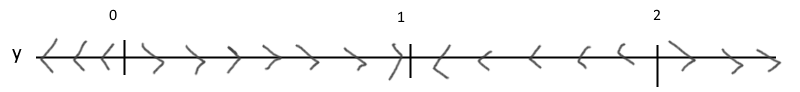
\includegraphics[width=5.5in]{3b.png}
    \item Use the phase diagram to give a rough sketch of the integral curves

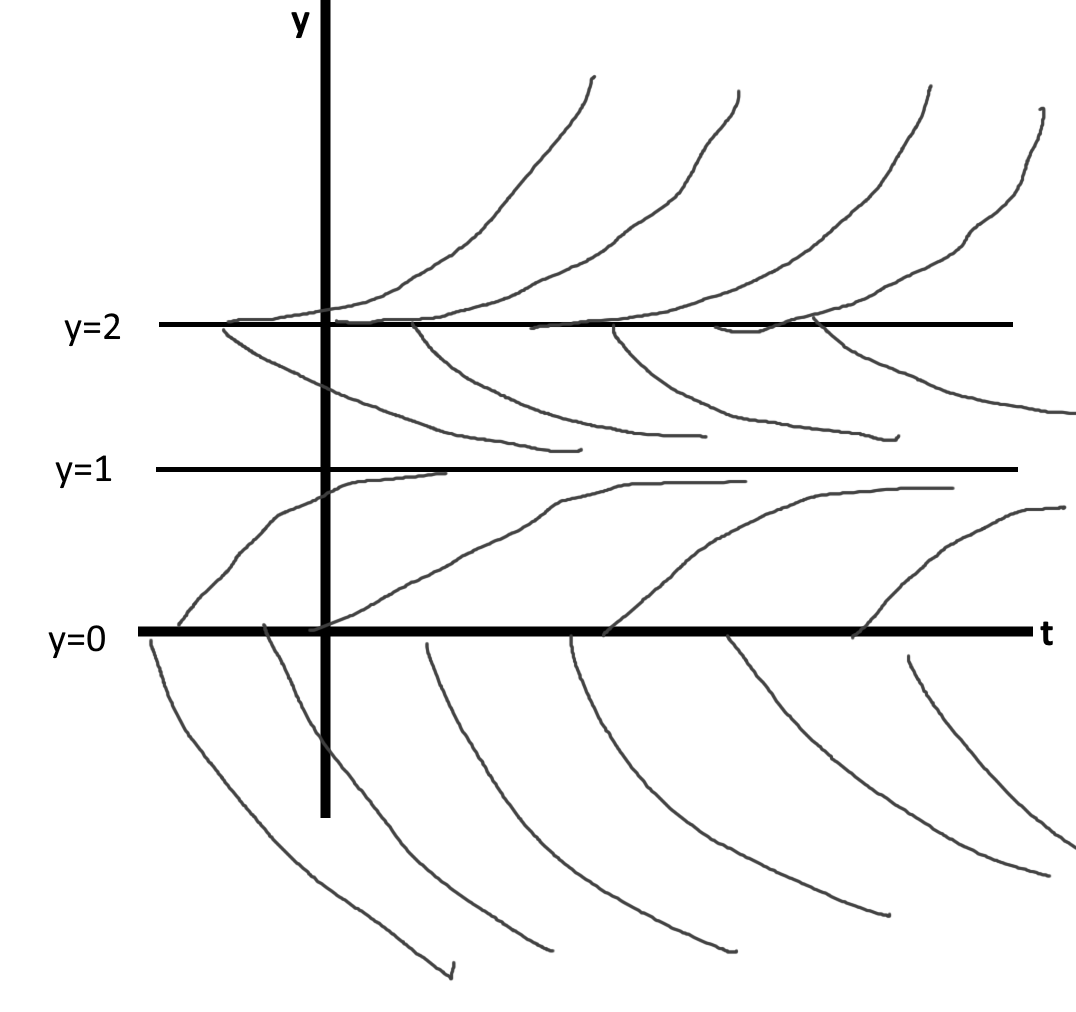
\includegraphics[width=4in]{3c.png}
\end{enumerate}\vspace{1cm}
    \item Find the general solution (by hand) of the differential equation 
$$y'' - y = \frac{2}{1+e^x}.$$

\soln First we solve the complementary equation $y'' - y = 0$. This is equivalent to $D^2 - I = 0$, which factors into $(D+I)(D-I)$. Thus the fundamental set is $\{e^{-x}, e^{x}\}$ and $$y_c = c_1 e^{-x} + c_2 e^x.$$
We want $Ly_p = \dfrac{2}{1+e^x}$ and $y_p = v_1 e^{-x} + v_2 e^{x}$. Therefore 
$${y_p}' = -v_1 e^{-x} + v_1'e^{-x} + v_2 e^x + v_2'e^x.$$
Here we assume $v_1'e^{-x} + v_2'e^x = 0$. Hence ${y_p}' = -v_1 e^{-x}  + v_2 e^x$. Therefore
$${y_p}'' = \underbrace{v_1 e^{-x} + v_2 e^x}_{y_p} - v_1' e^{-x} + v_2'e^x.$$
It follows that 
$${y_p}'' - y_p = - v_1' e^{-x} + v_2'e^x = \frac{2}{1+e^x}.$$
We now have a system of equations,
\begin{align*}
    \underbrace{\begin{bmatrix}
        e^{-x} & e^x \\ -e^{-x} & e^x
    \end{bmatrix}}_{:= A} \vvec*{v_1'}{v_2'}  &= \vvec*{0}{2/(1+e^x)}
\end{align*}
Note that $\det A =  W(e^{-x}, e^x) = 2$ and $A^{-1} = \dfrac{1}{\det A} \bigbrac{ (\operatorname{tr}A)I - A} = \dfrac{1}{2} \displaystyle \begin{bmatrix}
    e^x & -e^x \\ e^{-x} & e^{-x}
\end{bmatrix}$

\nl Multiplying by $A^{-1}$ on each side yields
\begin{align*}
    \vvec*{v_1'}{v_2'} &= \dfrac{1}{2} \displaystyle \begin{bmatrix}
        e^x & -e^x \\ e^{-x} & e^{-x}
    \end{bmatrix}  \vvec*{0}{2/(1+e^x)}\\
    &= \begin{bmatrix}
        \dfrac{-e^x}{1+e^x} & \dfrac{e^x}{1+e^x}
    \end{bmatrix}^T
    \\ & \\
    v_1' &= \dfrac{-e^x}{1+e^x} \\
    \int v_1' \dd x &= - \int \dfrac{e^x}{1+e^x} \dd x\\
    v_1 &= - \int \frac{\dd u}{u} \tag{Let $u = 1+e^x$}\\
    v_1 &= -\ln \abs{1+e^x} \\ & \\
    v_2' &= \dfrac{e^x}{1+e^x} \\
    v_2 &= \ln \abs{1+e^x}
\end{align*}
Substituting these functions into $y_p = v_1 y_1 + v_2 y_2$ yields
$$y_p = -e^{-x} \ln \abs{1+e^x} + e^x \ln \abs{1+e^x}.$$
The general solution $y = y_c + y_p$ is 
$$\boxed{$$y(x) = c_1 e^{-x} + c_2 e^{x} - e^{-x} \ln \abs{1+e^x} + e^x \ln \abs{1+e^x}$$}$$
% //


% \\
%     \vvec*{0}{2/(1+e^x)} &= \newpage
    \item Consider the non-homogeneous ODE
$$y''' + \over{x} y'' - \frac{2}{x^2}y' + \frac{2}{x^3}y = 2x.$$
\begin{enumerate}[label=(\alph*)]
    \item Verify that $\{x, x^2, 1/x\}$ form a fundamental set to the corresponding complementary ODE. 

\soln Let $y_1 := x$, $y_2 := x^2$, and $y_3 := 1/x$. Computing the Wronskian,
\begin{align*}
    W(y_1, y_2, y_3) &= \dety{x}{x^2}{x^{-1}}{1}{2x}{-x^{-2}}{0}{2}{2x^{-3}}\\
    &= x \detx{2x}{-x^{-2}}{2}{2x^{-3}} - x^2 \detx{1}{-x^{-2}}{0}{2x^{-3}} + x^{-1} \detx {1}{2x}{0}{2}\\
    &= 6/x - 2/x + 2/x\\
    &= 6/x
\end{align*}
Since the Wronskian is not zero, the set is linearly independent and 3 vectors in a third-order ODE span $\ker L$, thus forming a basis.

\newpage
    \item Determine a particular solution of the non-homogeneous ODE.

\soln* For a particular solution we need 
$$\bmaty{x}{x^2}{x^{-1}}{1}{2x}{-x^{-2}}{0}{2}{2x^{-3}} \vvec*{{v_1}'}{{v_2}'}{{v_3}'} = \vvec*{0}{0}{2x}.$$
Using Cramer's rule, 
\begin{align*}
    {v_1}' &= W^{-1}(y_1, y_2, y_3) \dety{0}{x^2}{x^{-1}}{0}{2x}{-x^{-2}}{2x}{2}{2x^{-3}} \\
    &= \frac{x}{6} \Bigbrac{ 0 - x^2(2x^{-1}) + x^{-1}(-4x^2) } \\
    &= -x^2\\
    \int {v_1}' \dd x &= \int -x^2 \dd x\\
    v_1(x) &= -\frac{1}{3}x^3\\
    &
    \\
    {v_2}' &= W^{-1}(y_1, y_2, y_3) \dety{x}{0}{x^{-1}}{1}{0}{-x^{-2}}{0}{2x}{2x^{-3}} \\
    &= \frac{x}{6} \Bigbrac{ x (2x^{-1}) - 0 + x^{-1}(2x) }\\
    &= \frac{2}{3}x\\
    \int {v_2}' \dd x &= \int \frac{2}{3}x \dd x\\
    v_2 &= \frac{1}{3}x^2\\
    &
    \\
    {v_3}' &= W^{-1}(y_1, y_2, y_3) \dety{x}{x^2}{0}{1}{2x}{0}{0}{2}{2x} \\
    &= \frac{x}{6} \Bigbrac{x(4x^2) -x^2 (2x) + 0}\\
    &= \frac 13 x^4 \\
    \int {v_3}' \dd x &= \int \frac 13 x^4 \dd x\\
    v_3 &= \frac{1}{15} x^5
\end{align*}
$y_p = v_1 y_1 + v_2 y_2 + v_3 y_3$ and thus $$\boxed{$$y_p(x)  = \dfrac{1}{15}x^4.$$}$$
\end{enumerate}
\end{enumerate}
\end{document} 